\subsection{Multi-environment Reinforcement Learning Post-training}
\label{subsec:multienvRL}
The Nemotron 3 models are designed to serve as the foundation for a wide variety of agentic AI applications. To teach Nemotron 3 the capabilities needed to succeed across such a broad range of tasks, we create a diverse set of reinforcement learning (RL) environments, covering mathematical and scientific reasoning, competitive coding, instruction following, software engineering, search, chat, general agentic tool use, long context, and more. Unlike our previous models where we had separate training stages for different tasks, we train the Nemotron 3 models on all of these tasks simultaneously. We find such simultaneous training is more stable, less prone to reward hacking and overall better compared to previous staged approaches \citep{basant2025nvidia}, which often results in degradation of some capabilities \citep{deepseekai2024deepseekv32}. The utility of multi-environment RL can be seen in Figure \ref{fig:multi-env-rl}, where performance on a wide variety of agentic and reasoning benchmarks steadily increases throughout Nemotron 3 Nano RL training.

\begin{figure}[]
    \centering
    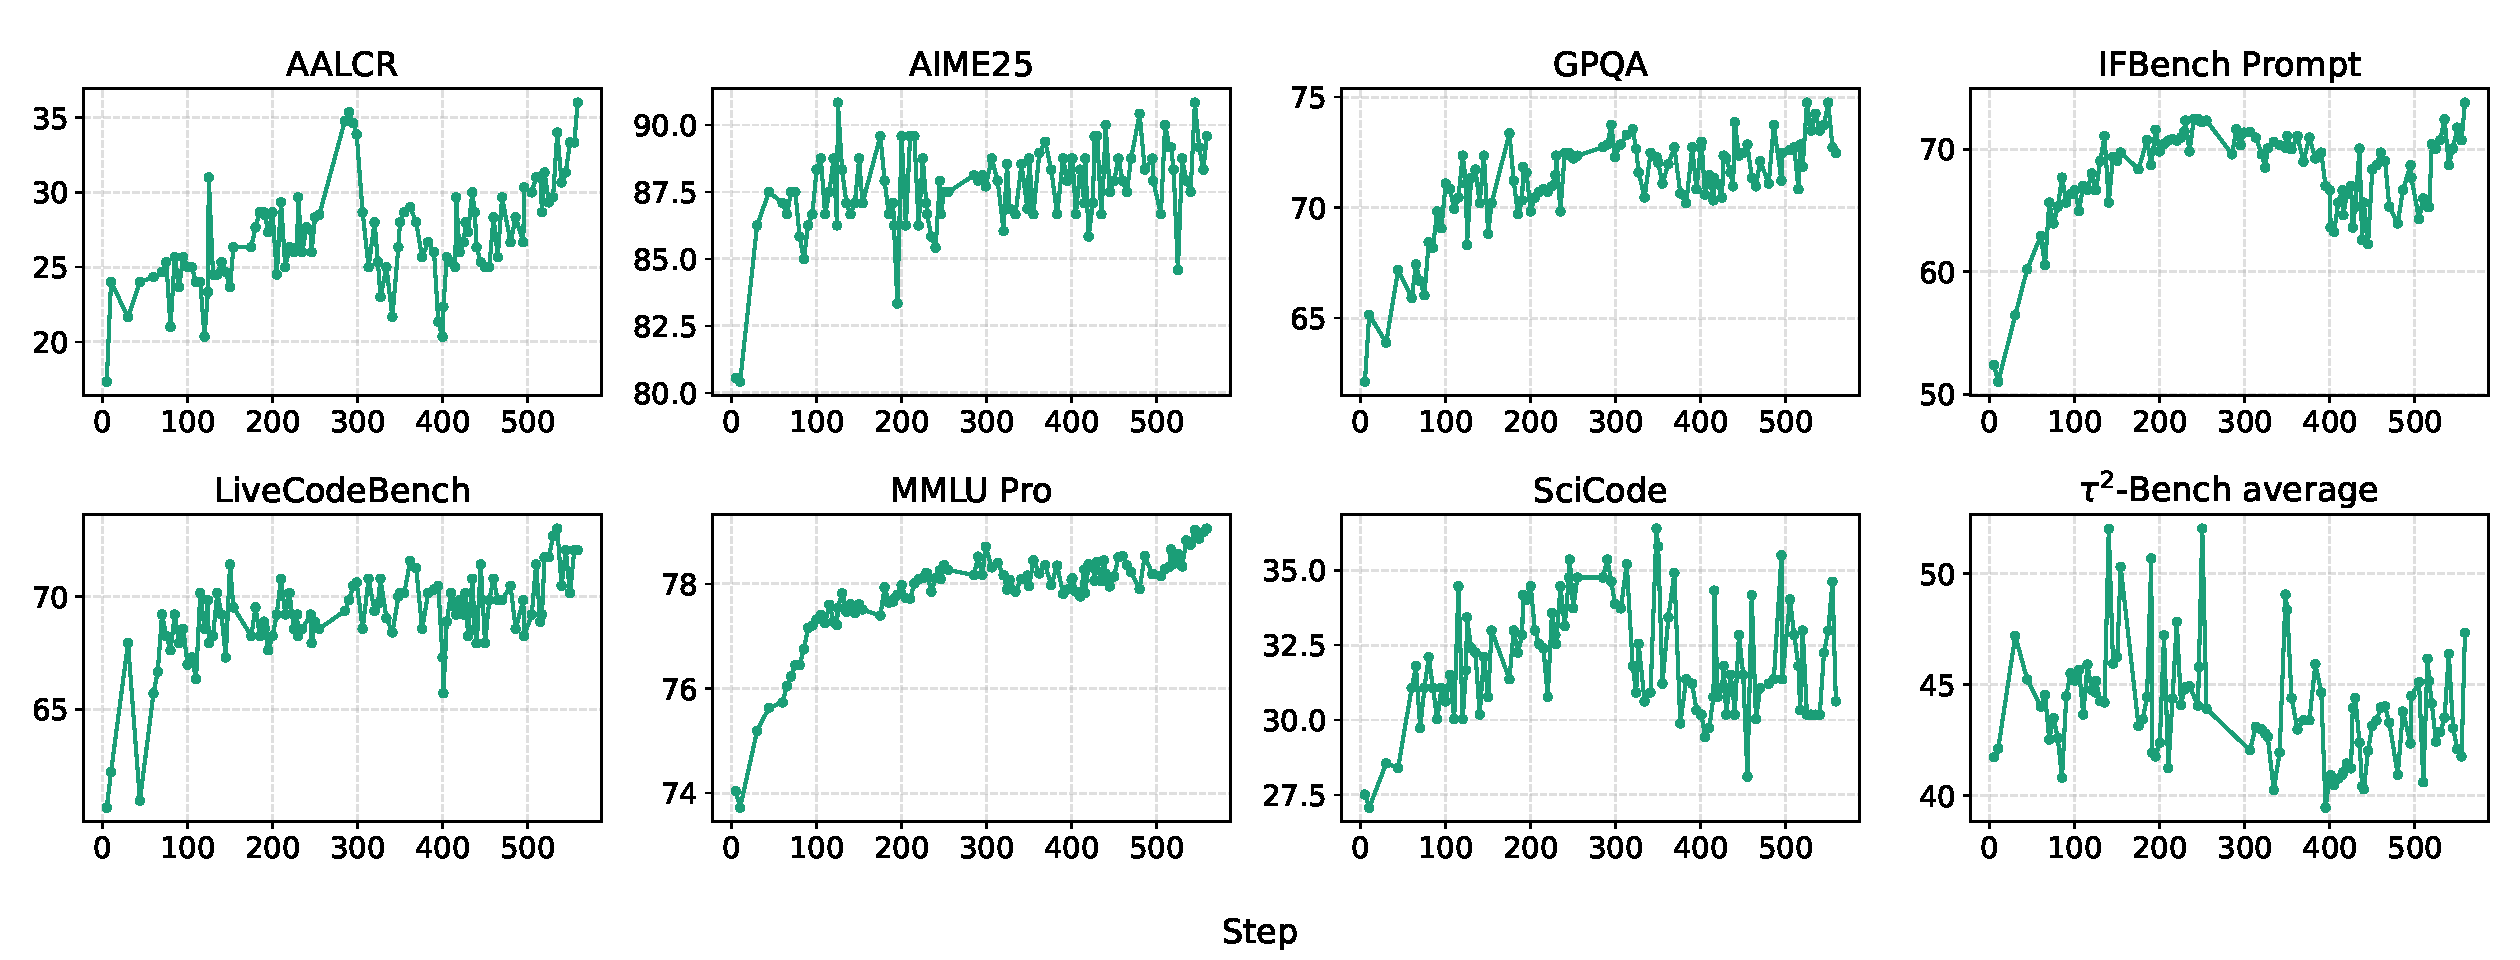
\includegraphics[width=0.9\textwidth]{figures/rl_progress_concat.pdf}
    \caption{Multi-environment RL training: within a single RL run several different environments corresponding to diverse capabilities are being optimized.
    }
    \label{fig:multi-env-rl}
\end{figure}

Large-scale RL across heterogeneous and complex environments requires efficient system design coupled with stable learning algorithms. The Nemotron 3 models are well suited for this setting, as their high inference throughput provides a significant advantage during large-scale rollout generation compared to other open-source models
% (total step time for Nemotron 3 Nano is roughly 40\% faster than Qwen3-30B-A3B in NeMo-RL)
. To further improve sampling efficiency, we employ an asynchronous RL architecture that decouples training from inference and leverage multi-token prediction to accelerate rollout generation. For stable training, we use GRPO \citep{deepseek-math} with masked importance sampling to account for discrepancies between the training and rollout policies.

Our entire post-training SW stack is open-sourced under Apache 2.0. NeMo-RL \footnote{\url{https://github.com/NVIDIA-NeMo/RL}} implements scalable RL training while NeMo-Gym \footnote{\url{https://github.com/NVIDIA-NeMo/Gym}} provides collection of RL environments.

% a high performance, extensible, and standardized interface for coordinating between rollouts and training.
% To address the extensibility challenges using one standard framework, we adopt NeMo Gym \citep{nemo-gym} and NeMo RL \citep{nemo-rl} for enabling large-scale RL on many different environments/verifiers. To improve the scalability of RL training, we adopt a variety of techniques, including asynchronous RL and low precision inference. 

% NeMo Gym is based on the abstraction of \emph{servers}.
% There are three core varieties of servers in Gym: (1) \emph{agents}, (2) \emph{models}, and (3) \emph{resources}.
% An \emph{agent} server implements the rollout kernel of a RL environment.
% A \emph{model} server wraps an inference engine to provide a prompt-response API, and also carefully preserves token and inference log-prob data and metadata required for RL.
% A \emph{resource} server provides a verification API for computing rewards from a given rollout.

% use multi-environment reinforcement learning. Different from our previous models we combine RL into a single training stage including all of our environments, which we find results in more stable training.
% We post-train our models via multi-environment reinforcement learning training. Different from our previous models we combine RL into a single training stage including all of our environments, which we find results in more stable training.

% To enable robust performance across a multitude of tasks, we 

\subsection{Granular Reasoning Budget Control at Inference Time}
\label{subsec:budgetcontrol}

Similar to Nemotron 2 Nano~\citep{basant2025nvidia}, the Nemotron 3 models are trained to work with inference-time budget control. Given a user-specified budget on the max number of tokens to use in a thinking trace and when the model reaches the budget, one can append the \texttt{</think>} token to the sequence and let the model continue to generate. The model will generate the response based on the partial thinking trace. Figure~\ref{fig:budgets} illustrates the accuracy-efficiency trade-off curves of Nemotron 3 Nano by varying the token budget, and this provides users fine-grained control in AI applications.

\begin{figure}[]
    \centering
    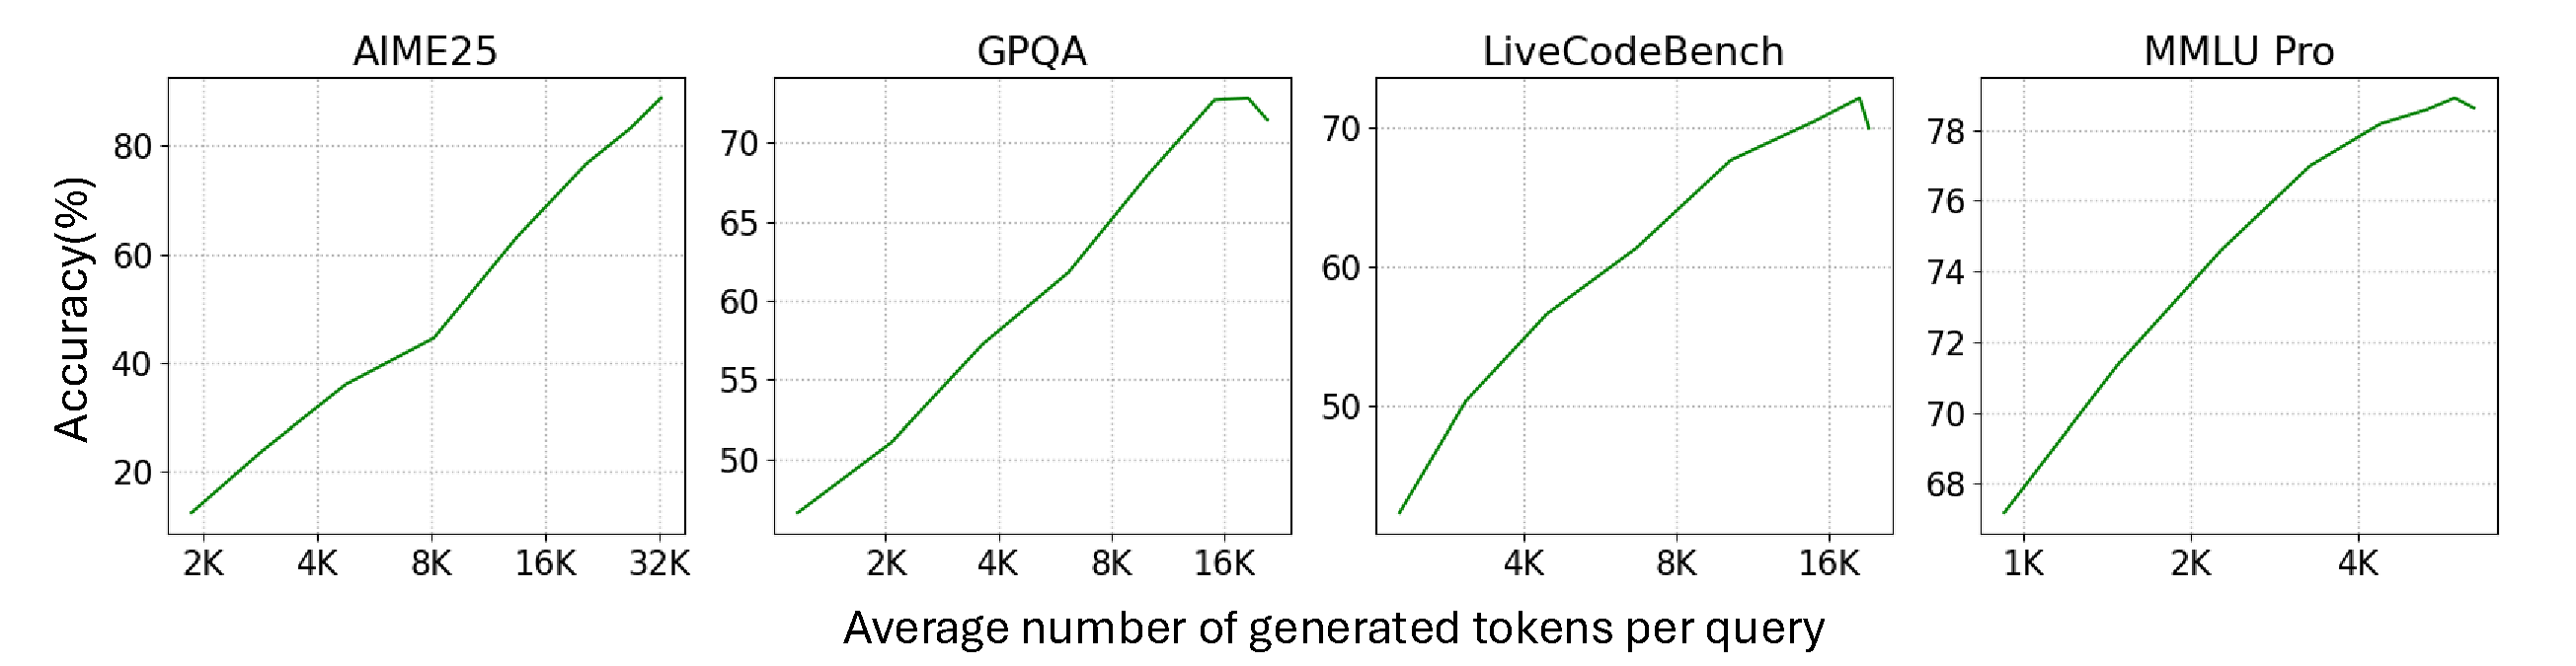
\includegraphics[width=0.9\textwidth]{figures/budgets4.pdf}
    \caption{Accuracy-efficiency trade-off with reasoning budget control at inference time.
    }
    \label{fig:budgets}
\end{figure}
